% Session 7 -- the area law, from the exactly solvable dimer and tetramer models.
% Placement: sec. "Two dimensions and the area law", after the dimer/tetramer comparison.
% Rendered by figures/blender/s07f02_arealaw.py, labels in figures/overlays/s07f02_arealaw.tex.
\begin{aqmfigure}{fig:s07:arealaw}{Why the entanglement entropy counts the boundary and not the
volume, seen from above. In both panels the ground state is an exact product of the ground states of
decoupled clusters, so a cluster that is fully inside $A$ or fully inside $B$ is in a pure state and
gives nothing. Only the clusters that are cut by the division contribute, and the cut bonds are the
red ones. (a) The dimerized chain. Each cut singlet gives exactly the single-dimer result $\log 2$
of (7.7), and the boundary of a block is two points for any length of the block. Each end of $A$
cuts through one dimer, so making $A$ larger, from two interior dimers to five, leaves two cut
singlets and $S_A = 2\log 2$ unchanged. The entropy saturates. (b) The same construction with
clusters of four sites on a square lattice. Each cluster that crosses the boundary still gives a
bounded amount, at most $\log 2$ per cut bond, but now the boundary is a curve whose length grows
with the subsystem. When we double the linear size of $A$, the number of cut bonds doubles, from
eight to sixteen, and $S_A$ grows in proportion. This is the area law (7.9), $S_A \sim
\alpha\,|\partial A|$, and the contrast between the two panels is the reason why matrix product
states are a one-dimensional tool.}
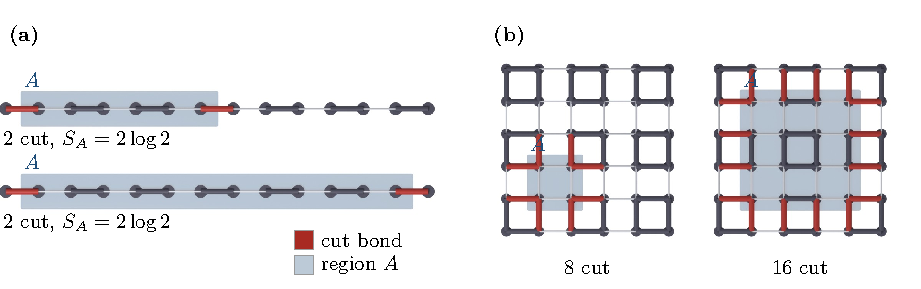
\includegraphics{figures/pdf/s07f02_arealaw.pdf}
\end{aqmfigure}
